\documentclass[a4paper]{article}

\usepackage[spanish]{babel}
\usepackage{graphicx}
\usepackage{amsmath, amssymb}
\usepackage[margin=2cm]{geometry}
\usepackage{fancyhdr}
\usepackage{enumerate}
\usepackage[shortlabels]{enumitem}
\usepackage{parskip}
\usepackage[most]{tcolorbox}
\usepackage[hidelinks]{hyperref}
\usepackage{float}


% cabecera
\pagestyle{fancy}
\fancyhead[l]{Daniel Soto}
\fancyhead[c]{Problemas de Astronomía \#3}
\fancyhead[r]{\today}
\fancyfoot[c]{\thepage}
\renewcommand{\headrulewidth}{0.2pt} % linea horizontal

\newcounter{problema}

\newtcolorbox[use counter=problema]{problema}[1][]{%
    colback=gray!15,
    colframe=gray!60,
    fonttitle=\bfseries,
    title={Problema~\theproblema:},
    boxrule=0.5mm,
    arc=3mm,
    boxsep=5pt,
    left=8pt,
    right=8pt,
    top=6pt,
    bottom=6pt,
    #1
}


\begin{document}

\begin{problema}
    
    \begin{figure}[H]
        \centering
        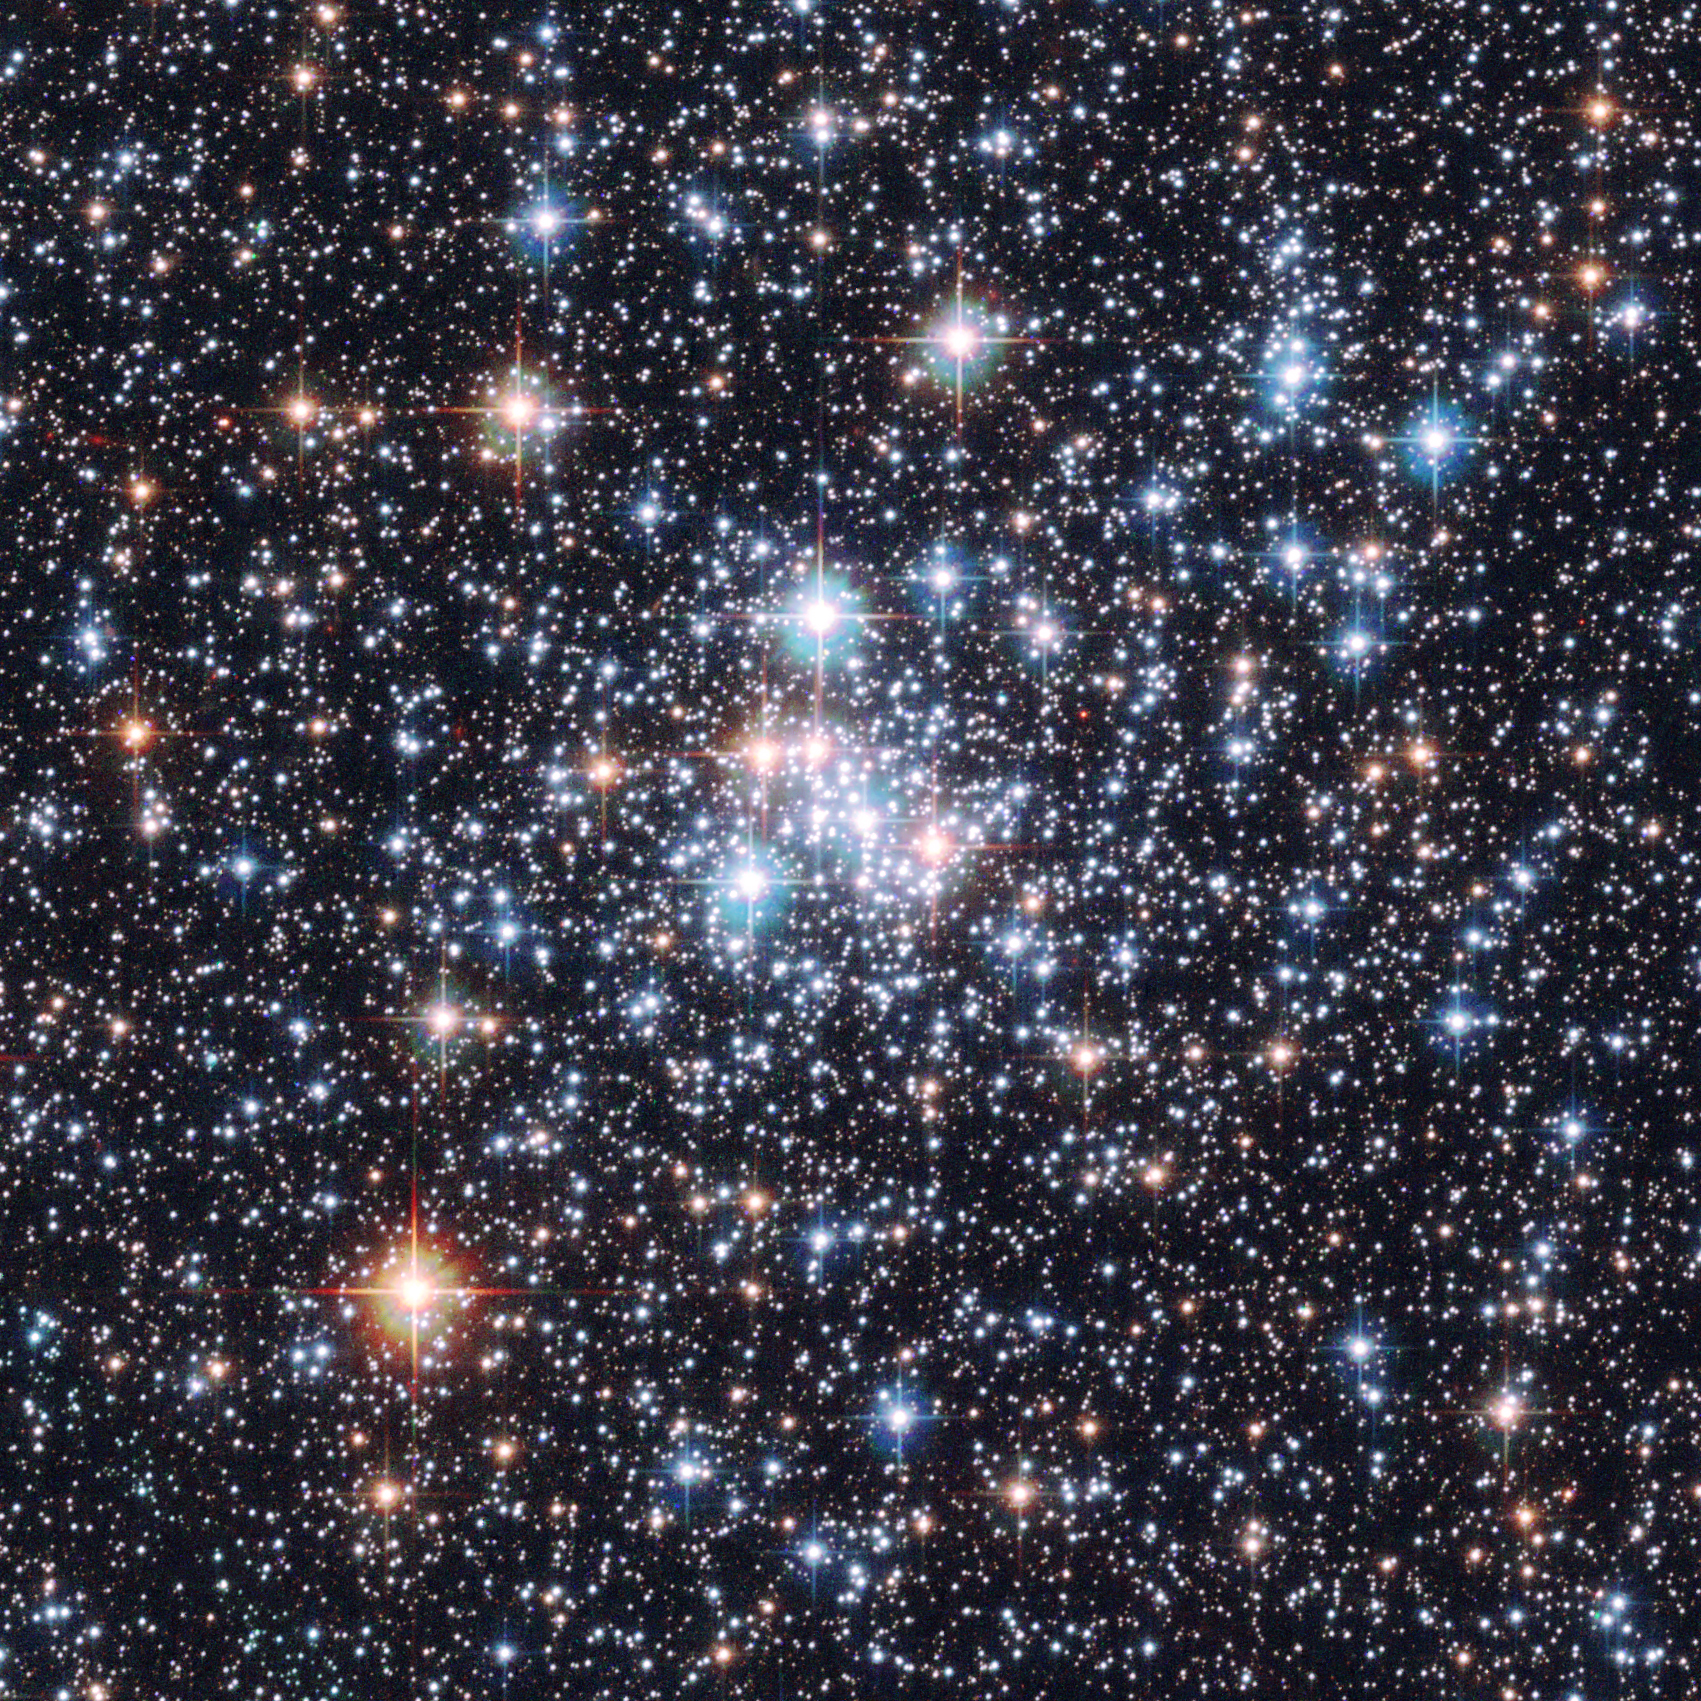
\includegraphics[width=0.5\textwidth]{StarCluster.jpg}
        \caption{Telescopio espacial Hubble: Cúmulo Estelar NGC 290}
        \label{fig:1}
    \end{figure}
    \textbf{Cúmulos estelares:} Como se muestra en la Figura \ref{fig:1}, consisten en cientos de estrellas que se mueven por el 
    espacio como una sola unidad.
    
    Los astrónomos necesitan conocer las masas de estos cúmulos, junto con la cantidad los diferentes tipos de estrellas que 
    los componen, para estudiar cómo se forman y cambian los cúmulos estelares con el tiempo.
    
    El cúmulo estelar NGC-290, mostrado en la foto del Telescopio Espacial Hubble, se encuentra en la galaxia cercana llamada 
    Nube Menor de Magallanes, a unos 200000 años luz de la Tierra.
    
    Los astrónomos utilizan la masa de nuestro Sol como una unidad conveniente de masas al comparar otras estrellas 
    ¡1 masa solar $[M_\odot]$ equivale a aproximadamente 2000 billones de toneladas! \cite{algebra2}
    \vspace{5mm}
	\begin{enumerate}
		\item Supongamos que NGC-290 tiene una masa total de no más de 500 $M_\odot$. 
		Si está compuesto por estrellas azules gigantes luminosas de tipo B con masas individuales de 10 $M_\odot$, 
		y estrellas rojas supergigantes antiguas de tipo M con masas individuales de 30 $M_\odot$, grafique una desigualdad 
		que muestre el número de estrellas B y M en este cúmulo. Escriba una desigualdad que represente esta información 
		y resuélvala gráficamente.
	
	    \item ¿La combinación de 9 estrellas de tipo B y 32 estrellas de tipo M conduce a una solución de población posible para este cúmulo?
	\end{enumerate}
\end{problema}
[2.6.1]

\begin{problema}
	El universo ha pasado por tres etapas diferentes de expansión poco después de Big Bang. 
	Los astrónomos llaman a estas etapas: \textit{Era Inflacionaria}, \textit{Era de Radiación} y \textit{Era de Materia}.
	
	\begin{figure}[H]
	        \centering
	        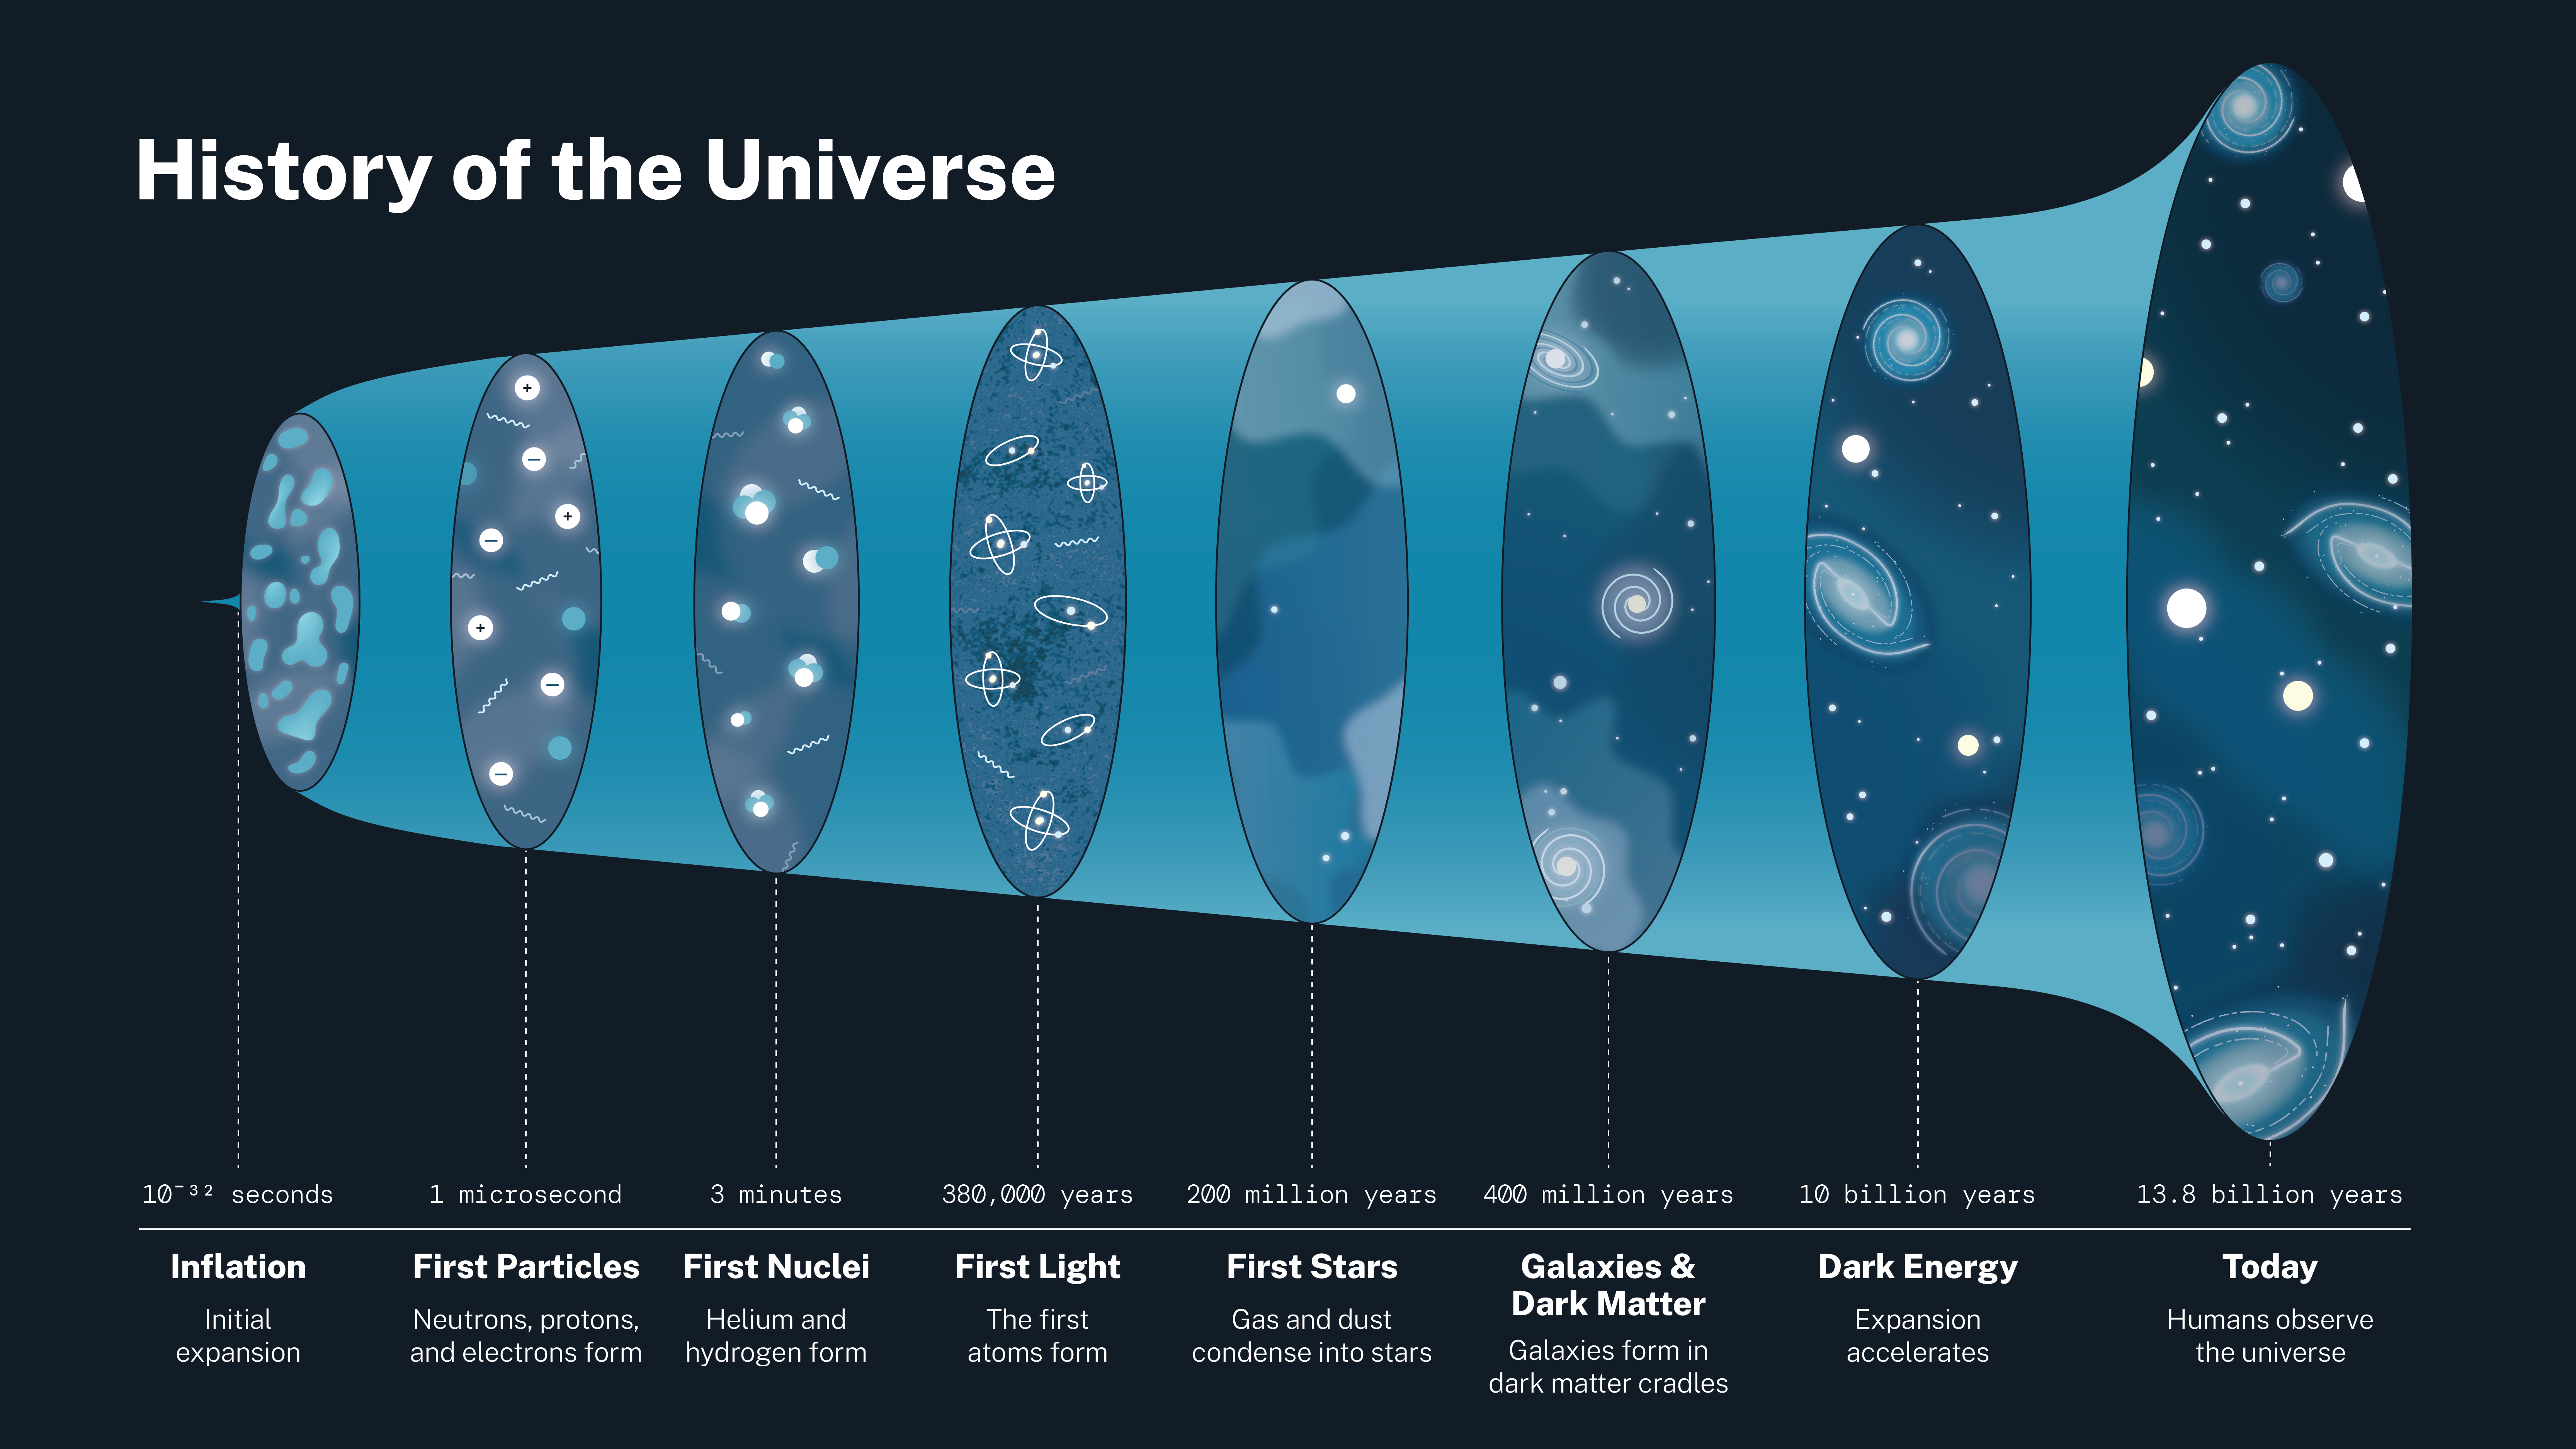
\includegraphics[width=\textwidth]{CosmicEpochs.png}
	        \caption{Diferentes épocas cósmicas}
	        \label{fig:2}
	\end{figure}
	El tamaño del universo está determinado por las separaciones entre objetos típicos, y puede representarse 
	mediante modelos matemáticos basados en las ecuaciones físicas que rigen el comportamiento de la materia, 
	la energía y la gravedad.
	
	La expansión del universo puede definirse mediante la siguiente función definida a trozos, donde la variable $t$ 
	se mide en segundos desde el Big Bang:
	
	$$ a(t) = \left\{\begin{matrix}
	2.2\times 10^{-29}e^{10^{35t}} & 10^{-35} < t < 10^{-33} \quad\text{Era de Inflación} \\
	6.4\times 10^{10}\sqrt{t} & 10^{-33} < t < 9.3\times 10^{12} \quad\text{Era de Radiación} \\
	7700 t ^ {4/3} & 9.3\times 10^{12} < t < 4.2\times 10^{17} \quad\text{Era de la Materia}
	\end{matrix}\right.$$
	\vspace{5mm}
	\begin{enumerate}
		\item ¿Cuál es la gráfica de $a(t)$ entre 1 segundo y 10 minutos después del Big Bang?
	
		\item ¿Cuál es la gráfica de $a(t)$ entre 12 y 13 mil millones de años después del Big Bang?
	
		\item ¿En qué factor cambia $a(t)$ cuando el tiempo trancurrido desde el Big Bang aumenta en un factor de 10 durante cada era?
	\end{enumerate}
\end{problema}
[2.7.1]


\begin{problema}
	\begin{figure}[H]
	        \centering
	        \includegraphics[width=\textwidth]{VerticalMotionGravity.jpeg}
	        \caption{Marte, Luna y Tierra}
	        \label{fig:3}
	\end{figure}

	\textbf{Movimiento vertical bajo la gravedad:} La expresión común 'lo que sube, debe bajar' puede representarse mediante 
	una ecuación cuadrática. Si trazara la altura de una pelota lanzada verticalmente, su altura en función del tiempo seguiría 
	una sencilla fórmula cuadrática dada por la ecuación general:

	$$H(t) = h_0 +vt - \frac{1}{2}g t^2$$

	donde $h_0$ es la altura inicial de la pelota en metros, $v$ es la velocidad inicial en $\text{m/s}$, y $g$ es la 
	aceleración de la gravedad en $\text{m/s}^2$. Es una ecuación general porque funciona no solo en la Tierra, 
	sino también en casi todos los demás cuerpos astronómicos, excepto en los agujeros negros. Para los agujeros negros, 
	la geometría del espacio está tan distorsionada que $t, v$ y $h_0$ se alteran de formas complejas.

	\vspace{5mm}

	Para los siguientes problemas:

	\vspace{5mm}

	\begin{itemize}
		\item Escriba la ecuación en forma estándar.

		\item Determine las coordenadas del vértice de la parábola donde $H(t)$ es máximo.

		\item Determine el eje de simetría.

		\item En una misma gráfica para los tres problemas, trace la parábola para cada problema 
		graficando dos puntos adicionales utilizando la propiedad del eje de simetría, para todos los 
		tiempos positivos durante los cuales $H(t)>0$
	\end{itemize}
	
	\vspace{5mm}

	\begin{enumerate}
		\item En la Tierra, la aceleración de la gravedad es $g=10 \text{ m/s}^2$. 
		La pelota fue lanzada verticalmente hacia arriba con una velocidad inicial 
		de $v=20\text{ m/s}$ desde una altura de $h_0=2\text{ m}$.
	
		\item En Marte, la aceleración de la gravedad es $g=4 \text{ m/s}^2$. 
		La pelota fue lanzada verticalmente hacia arriba con una velocidad inicial 
		de $v=20\text{ m/s}$ desde una altura de $h_0=2\text{ m}$.

		\item En la Luna, la aceleración de la gravedad es $g=2 \text{ m/s}^2$. 
		La pelota fue lanzada verticalmente hacia arriba con una velocidad inicial 
		de $v=20\text{ m/s}$ desde una altura de $h_0=2\text{ m}$.
	\end{enumerate}
\end{problema}
[5.1.1]
\bibliographystyle{plainurl}
\bibliography{bibliografia} % Nombre del .bib

\end{document}
